\header{
    \section{Quand je bois du vin clairet} \label{quand-je-bois-du-vin-clairet}
    %
    \insertComment{Le vin clairet est un vin un peu plus tanique que le rosé, mais pas tout à fait autant qu’un rouge.}{Editée par Pierre Attaingnant vers 1530.}
}

\enluminure{4}{\href{https://www.youtube.com/watch?v=rxlwCTOuTSs}{Q}}~\\
$\left.\begin{tabular}{l}
\hspace{-0.4cm}
\textsc{uand} je bois du vin clairet,
\\
\hspace{-0.4cm}
Ami tout tourne, tourne, tourne, tourne...
\\
\hspace{-0.4cm}
Aussi désormais 
\\
\hspace{-0.4cm}
Je bois Anjou ou Arbois.
\end{tabular}\right\rbrace$ bis\\\\
\bisquadruplespace{Chantons et buvons}
{À ce flacon faisons la guerre!}
{Chantons et buvons}
{Mes amis; buvons donc!}
\bisquadruplespace{De ce gras jambon}
{Mangeons pour oublier nos peines!}
{De ce gras jambon}
{Mes amis, mangeons donc!}
\bisquadruple{Chantons et buvons}
{Vive l'amour et la bouteille!}
{Chantons et buvons}
{Mes amis; buvons donc!}

\vspace{0.5cm}

\begin{center}
   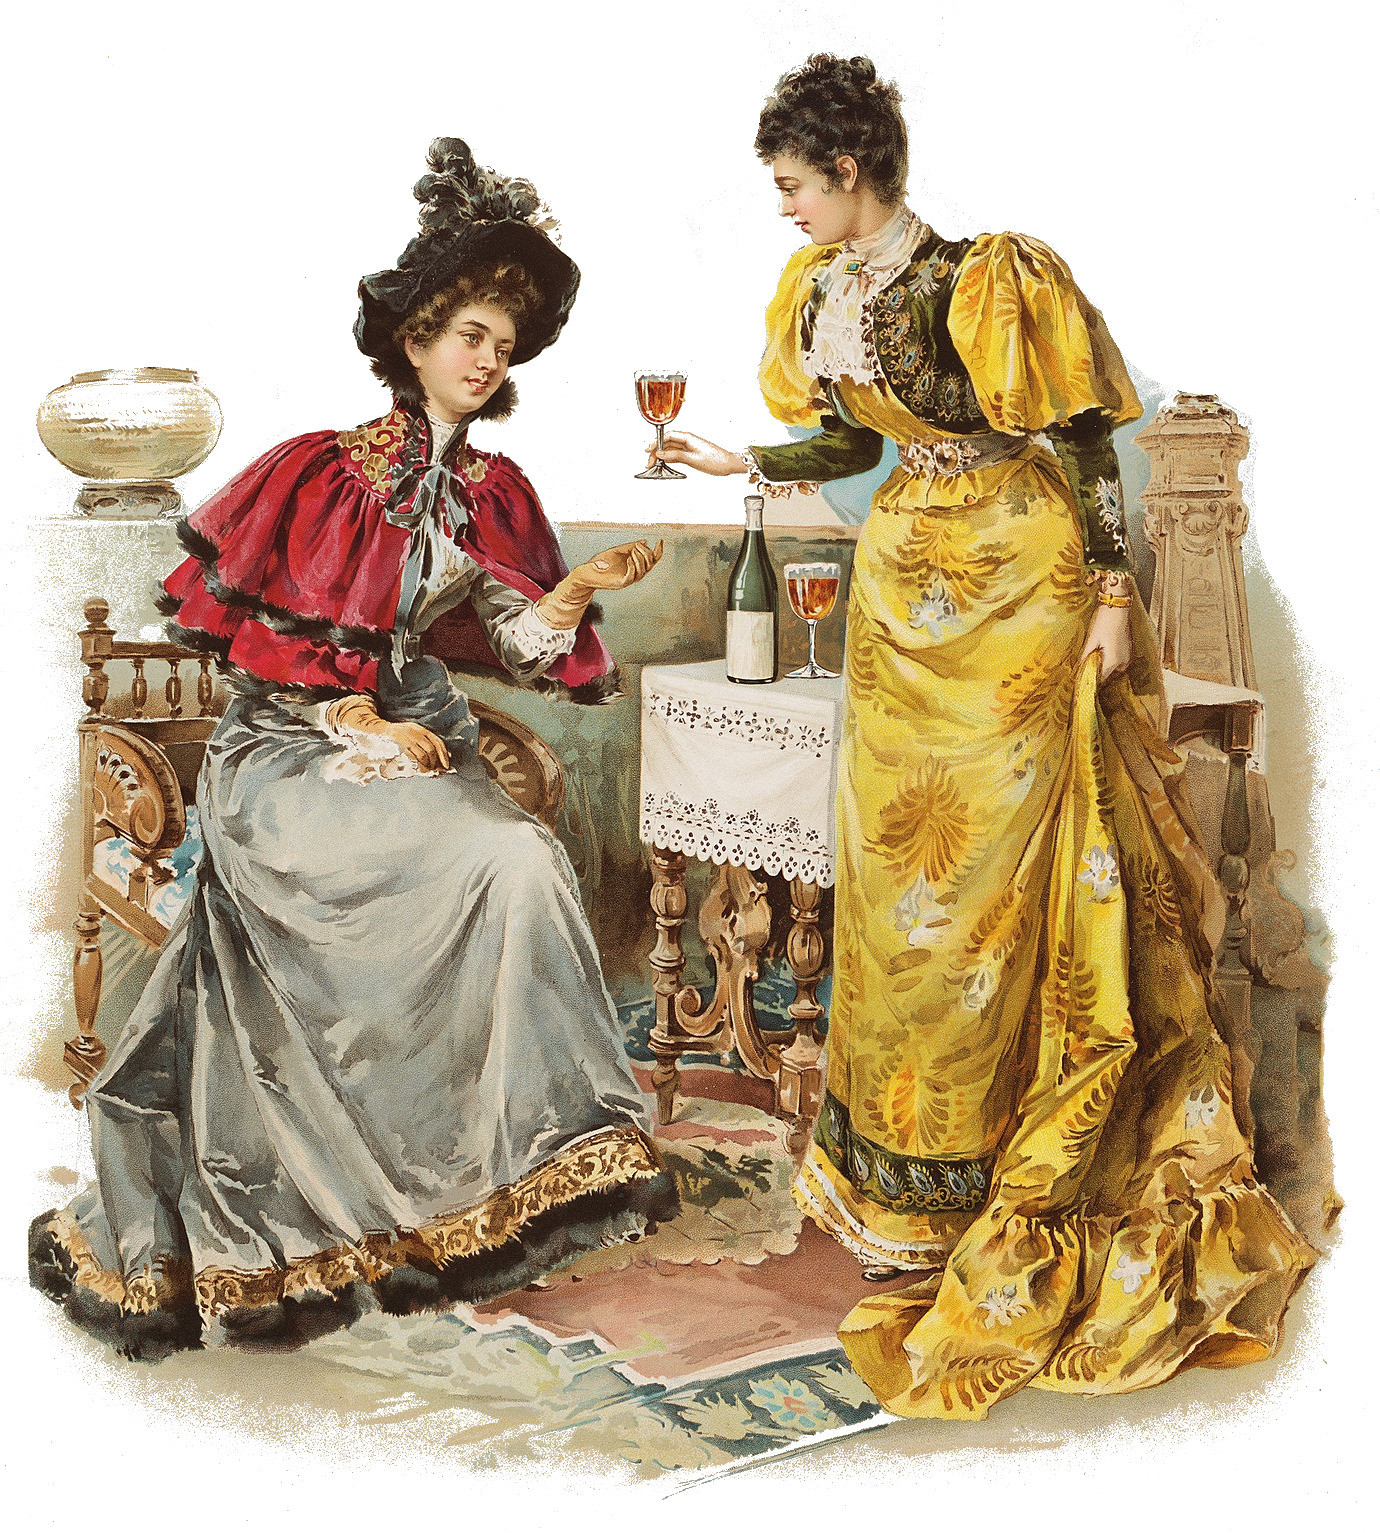
\includegraphics[width=0.4\textwidth]{images/brev85.png}
 \end{center}
\breakpage